\sec{Case study}
\ssec{Introduction}

\begin{frame}{Sustainable land management} 
\i Agriculture faces complex challenges to satisfy a population of $9\cdot10^9$ (2050)
\i More water is needed to produce the estimated 60\% of extra food
\i FAO\footnote{\url{http://www.fao.org/water/en/}}: we need a more efficient use of water

\begin{block}{Sustainable land management (United Nations)}
Use of land resources, including soils, water, animals and plants, for the production of goods to meet changing human needs, while simultaneously ensuring the long-term productive potential of these resources and the maintenance of their environmental functions
\end{block}
\end{frame}

\begin{frame}{Scenario}
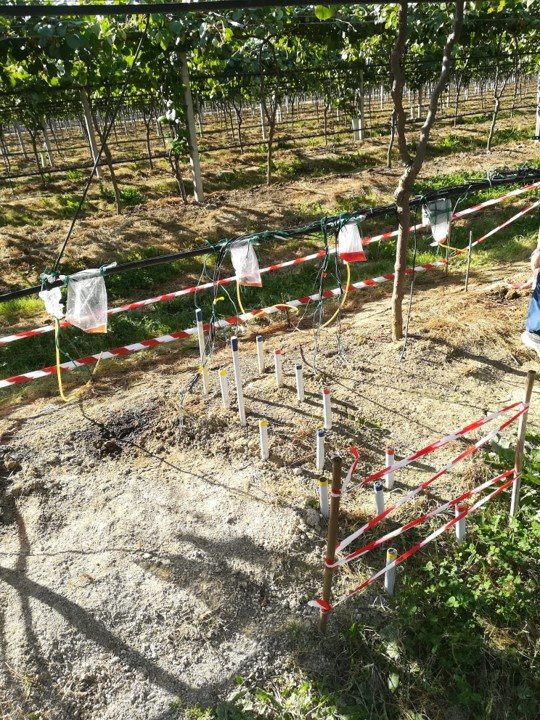
\includegraphics[height=.8\textheight]{imgs/casestudy_real.jpg}
\end{frame}

\begin{frame}{Scenario: water propagation}
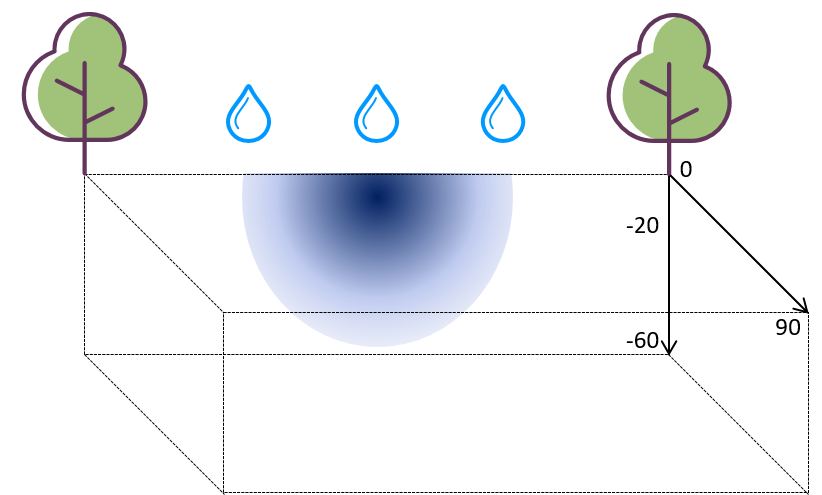
\includegraphics[width=.6\textwidth]{imgs/casestudy.png}
\end{frame}

\begin{frame}{Scenario}
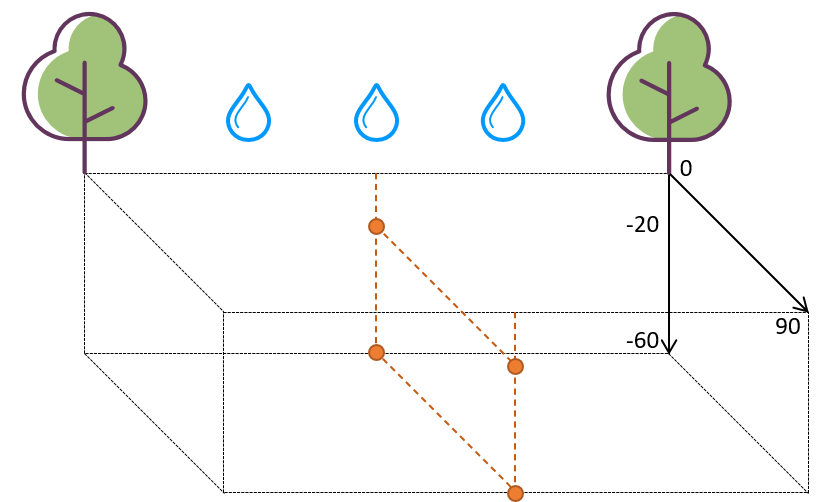
\includegraphics[width=.6\textwidth]{imgs/casestudy_sensors.png}
\end{frame}

\begin{frame}{Smart irrigation: humidity sensors}

\textbf{Goal}: optimization of water resources, provide water only if necessary

\textbf{How}: given humidity sensors displaced on the field, alert the farmer when there is need for irrigation

\textbf{How (technically)}:

\i \textbf{collect} and \textbf{store} raw data from the sources
\i interpolate raw data and \textbf{store} new nata
\i \textbf{alert} when the soil is *too dry*
\i make data available to \textbf{dashboards}
\i ...

\end{frame}

\begin{frame}{Smart-irrigation data pipeline}

\begin{block}{Data pipeline}
Sequences of actions that extract data (or directly analytics and visualization) from various sources
\end{block}

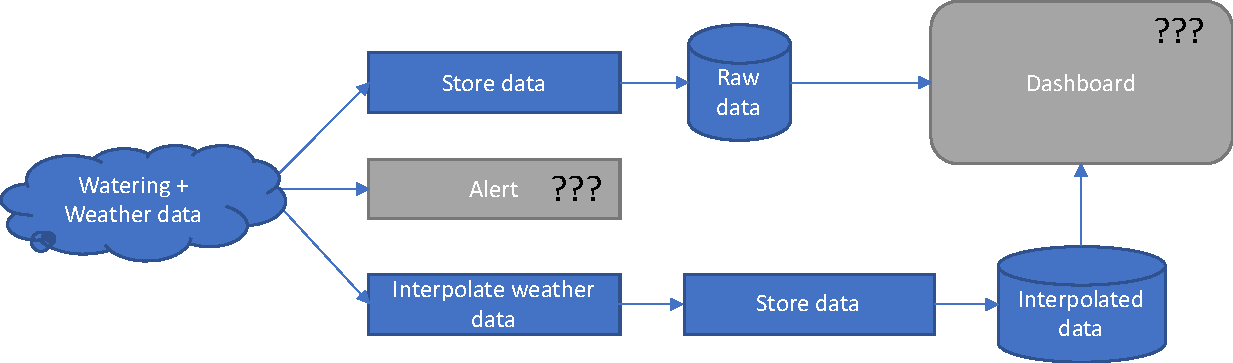
\includegraphics[width=\linewidth]{imgs/pipeline.pdf}
\end{frame}

\begin{frame}{Issues}
\i Building blocks
\i Heterogeneity and compatibility
\end{frame}

\begin{frame}{Issue: building blocks (services)}

\end{frame}